\section{Métodos de Runge-Kutta}

\subsection{Introdução}

Problema

\begin{equation}
 \label{cap6:sec3:eq1}
 \begin{array}{l}
  u' = f \, (u, \, t) \\
  u \, (0) = u_0
 \end{array}
\end{equation}

no intervalo $ \, [t_n, \, t_{n+1}] \, $

\begin{equation}
 \label{cap6:sec3:eq2}
 u_{n+1} = u_n + \int^{\,t_{n+1}}_{t_n} f \, (v, \, t) \, dt
\end{equation}

Os métodos de Runge-Kutta são derivados aplicando-se integração numérica para aproximar a integral em \ref{cap6:sec3:eq2}.

\begin{equation}
 \label{cap6:sec3:eq3}
 I = \int^{\,t_{n+1}}_{t_n} f \, (v, \, t) \, dt
\end{equation}

\textbf{Regra do Trapézio} $ \, (\Delta t = h) $

\begin{equation}
 \label{cap6:sec3:eq4}
 I \approx \frac{h}{2} \, [f \, (v_n, \, t_n) + f \, (v_{n+1}, \, t_{n+1})]
\end{equation}

\textbf{Regra 1/3 de Simpson} $ \, (\bar{h} = h/2) $

\begin{figure}[htb]
 \centering
 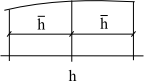
\includegraphics[scale=1.0]{capitulos/capitulo6/figuras/met_runge_kutta1.png}
 \caption{Regra de 1/3 de Simpson}
 \label{fig:met_runge_kutta1}
\end{figure}

\begin{equation}
 \label{cap6:sec3:eq5}
 I \approx \underbrace{\frac{\bar{h}}{3}}_{h/6} [f \, (v_n, \, t_n) + 4 \, f \, (v_{n+\frac{1}{2}}, \, t_{n+\frac{1}{2}}) + f \, (v_{n+1}, \, t_{n+1})]
\end{equation}

\textbf{Regra 3/8 de Simpson} $ \, (\bar{h} = h/3) $

\begin{figure}[htb]
 \centering
 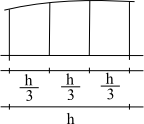
\includegraphics[scale=1.0]{capitulos/capitulo6/figuras/met_runge_kutta2.png}
 \caption{Regra de 3/8 de Simpson}
 \label{fig:met_runge_kutta2}
\end{figure}

\begin{equation}
 \label{cap6:sec3:eq6}
 I \approx \underbrace{\frac{3\bar{h}}{8}}_{h/9} [f \, (v_n, \, t_n) + 3 \, f \, (v_{n+\frac{1}{3}}, \, t_{n+\frac{1}{3}}) + 3 \, f \, (v_{n+\frac{2}{3}}, \, t_{n+\frac{2}{3}}) + f \, (v_{n+1}, \, t_{n+1})]
\end{equation}

Para obtermos os valores de $ \, f(v, \, t) \, $ nos pontos intermediários do intervalo basta obtermos os valores de $ \, v \, $ e $ \, t \, $ nos pontos intermediários. Isto é feito obtendo-se uma estimativa aplicando-se ``\textit{Forward} Euler''.

Assim,

\begin{eqnarray}
 \label{cap6:sec3:eq7}
 \bar{v}_{n+\frac{1}{2}} & = & v_n + \frac{h}{2} \, f \, (v_n, \, t_n) \\
 \label{cap6:sec3:eq8}
 \bar{v}_{n+\frac{1}{3}} & = & v_n + \frac{h}{3} \, f \, (v_n, \, t_n) \\
 \label{cap6:sec3:eq9}
 \bar{v}_{n+\frac{2}{3}} & = & v_n + \frac{2\,h}{3} \, f \, (v_n, \, t_n) \\
 \label{cap6:sec3:eq10}
 \bar{v}_{n+1} & = & v_n + h \, f \, (v_n, \, t_n)
\end{eqnarray}

\subsection{Runge-Kutta de Segunda Ordem}

Baseado na Regra do Trapézio

\begin{equation}
 v_{n+1} = v_n + \frac{h}{2} \, [f \, (v_n, \, t_n) + f(\bar{v}_{n+1}, \, t_{n+1})]
\end{equation}

onde $ \, \bar{v}_{n+1} = v_n + h \, f \, (v_n, \, t_n) \, $

chamando-se

\begin{eqnarray}
 \label{cap6:sec3:eq12}
 & & k_1 = h \, f \, (v_n, \, t_n) \\
 \label{cap6:sec3:eq13}
 & & \bar{v}_{n+1} = v_n + k_1 \\
 \label{cap6:sec3:eq14}
 & & k_2 = h \, f \, (v_n + k_1, \, t_{n+1})
\end{eqnarray}

temos

\begin{equation}
 \label{cap6:sec3:eq15}
 \mbox{ \framebox{ $ v_{n+1} = v_n + \frac{1}{2} \, [k_1 + k_2] $ } }
\end{equation}

\subsection{Runge-Kutta de Terceira Ordem}

Baseado na Regra 1/3 de Simpson

\begin{eqnarray}
 \label{cap6:sec3:eq16}
 && v_{n+1} = v_n + \frac{h}{6} \, [f \, (v_n, \, t_n) + 4 \, f \, (\bar{v}_{n+\frac{1}{2}}, \, t_{n+\frac{1}{2}}) + f \, (\bar{v}_{n+1}, \, t_{n+1})] \\
 \label{cap6:sec3:eq17}
 && \bar{v}_{n+\frac{1}{2}} = v_n + \frac{h}{2} \, f \, (v_n, \, t_n)
\end{eqnarray}

\begin{figure}[htb]
 \centering
 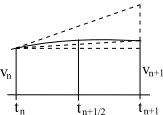
\includegraphics[scale=1.0]{capitulos/capitulo6/figuras/met_runge_kutta3.png}
 \caption{?}
 \label{fig:met_runge_kutta3}
\end{figure}

A estimativa $ \, \bar{v}_{n+1} \, $ pode ser obtida de várias maneiras

\begin{enumerar}


\item
\label{item.i}

\begin{equation}
 \label{cap6:sec3:eq18}
 \bar{v}_{n+1} = v_n + h \, f \, (v_n, \, t_n)
\end{equation}

\item
\label{item.ii}

\begin{equation}
 \label{cap6:sec3:eq19}
 \bar{v}_{n+1} = v_n + h \, f \, (\bar{v}_{n+\frac{1}{2}}, \, t_{n+\frac{1}{2}})
\end{equation}

\item Combinação linear de \ref{item.i} e \ref{item.ii}

\begin{equation}
 \label{cap6:sec3:eq20}
 \bar{v}_{n+1} = v_n + h \, [\theta \, f \, (v_n, \, t_n) + (1 - \theta) \, f \, (\bar{v}_{n+\frac{1}{2}}, \, t_{n+\frac{1}{2}})]
\end{equation}

O valor ótimo de $ \, \theta \, $ é $ \, \theta = -1 \, $. Assim

\begin{equation}
 \label{cap6:sec3:eq21}
 \bar{v}_{n+1} = v_n + h \, [-f \, (v_n, \, t_n) + 2 \, f \, (\bar{v}_{n+\frac{1}{2}}, \, t_{n+\frac{1}{2}})]
\end{equation}

\end{enumerar}

Chamando-se

\begin{eqnarray}
 \label{cap6:sec3:eq22}
 k_1 & = & h \, f \, (v_n, \, t_n) \\
 \label{cap6:sec3:eq23}
 \bar{v}_{n+\frac{1}{2}} & = & v_n + \frac{1}{2} \, k_1 \\
 \label{cap6:sec3:eq24}
 k_2 & = & h \, f \, (v_n + \frac{1}{2} \, k_1, \, t_n + \frac{h}{2}) \\
 \label{cap6:sec3:eq25}
 k_3 & = & h \, f \, (v_n - k_1 + 2 \, k_2, \, t_n + h)
\end{eqnarray}

\begin{equation}
 \label{cap6:sec3:eq26}
 \mbox{ \framebox{ $ v_{n+1} = v_n + \displaystyle \frac{1}{6} \, (k_1 + 4 \, k_2 + k_3) $ } }
\end{equation}


\subsection{Runge-Kutta de Quarta Ordem}

Baseado na Regra 3/8 de Simpson

\[
 v_{n+1} = v_n + \frac{h}{8} \, [f \, (v_n, \, t_n) + 3 \, f \, (\bar{v}_{n+\frac{1}{3}}, \, t_{n+\frac{1}{3}}) + 3 \, f \, (\bar{v}_{n+\frac{2}{3}}, \, t_{n+\frac{2}{3}}) + f(\bar{v}_{n+1}, \, t_{n+1})]
\]

Chamando-se

\begin{eqnarray}
 k_1 & = & h \, f \, (v_n , \, t_n) \nonumber \\
 \nonumber \\
 k_2 & = & h \, f \, \left(v_n + \frac{1}{3} \, k_1, \, t_n + \frac{h}{3}\right) \nonumber \\
 \nonumber \\
 \bar{v}_{n+\frac{1}{3}} & = & v_n + \frac{1}{3} \, k_1 \nonumber \\
 \nonumber \\
 \bar{v}_{n+\frac{2}{3}} & = & v_{n+\frac{1}{3}} + \frac{h}{3} \, f \, (\bar{v}_{n+\frac{1}{3}}, \, t_{n+\frac{1}{3}}) \nonumber \\
 \nonumber \\
 & = & v_n + \frac{1}{3} \, k_1 + \frac{1}{3} \, k_2 \nonumber \\
 \nonumber \\
 k_3 & = & h \, f \, \left(v_n + \frac{k_1}{3} + \frac{k_2}{3}, \, t_n + \frac{2 \, h}{3}\right) \nonumber \\
 \nonumber \\
 \bar{v}_{n+1} & = & v_n + h \, f \, (v_n) - h \, f \, (\bar{v}_{n+\frac{1}{3}}) + h \, f \, (\bar{v}_{n+\frac{2}{3}}) \nonumber \\
 \nonumber \\
 k_4 & = & h \, f \, (v_n + k_1 - k_2 + k_3, \, t_n + h) \nonumber 
\end{eqnarray}

\[
 \mbox{ \framebox{ $ v_{n+1} = v_n + \displaystyle \frac{1}{8} \, [k_1 + 3 \, k_2 + 3 \, k_3 + k_4] $ } }
\]


Derivem em casa a eq. 9.3.17 da página 330.